% ------------------------------------------------------------------------------
% TYPO3 CMS 7.6 - What's New - Chapter "Introduction" (English Version)
%
% @author	Michael Schams <schams.net>
% @license	Creative Commons BY-NC-SA 3.0
% @link		http://typo3.org/download/release-notes/whats-new/
% @language	English
% ------------------------------------------------------------------------------
% LTXE-CHAPTER-UID:		cb43d098-7bf9a537-bf3817c0-53a0f29f
% LTXE-CHAPTER-NAME:	Introduction
% ------------------------------------------------------------------------------

\section{Introduction}
\begin{frame}[fragile]
	\frametitle{Introduction}

	\begin{center}\huge{Introduction}\end{center}
	\begin{center}\huge{\color{typo3darkgrey}\textbf{The Facts}}\end{center}

\end{frame}

% ------------------------------------------------------------------------------
% LTXE-SLIDE-START
% LTXE-SLIDE-UID:		d2b92f95-205056c1-67c47efd-cc5156ac
% LTXE-SLIDE-ORIGIN:	9e397afb-762f7061-0e0e0bd1-9836250e English
% LTXE-SLIDE-ORIGIN:	1e50fa0a-e0f4c00a-5f667356-11df7c7c German
% LTXE-SLIDE-TITLE:		TYPO3 CMS 7.6 - The Facts
% ------------------------------------------------------------------------------
\begin{frame}[fragile]
	\frametitle{Introduction}
	\framesubtitle{TYPO3 CMS 7.6 - The Facts}

	\begin{itemize}
		\item Release date: 10 November 2015
		\item Release type:
			\begingroup\color{red}Long Term Support (LTS) Release\endgroup
		\item Vision: Embrace, Innovate, Deliver
	\end{itemize}

	\begin{figure}
		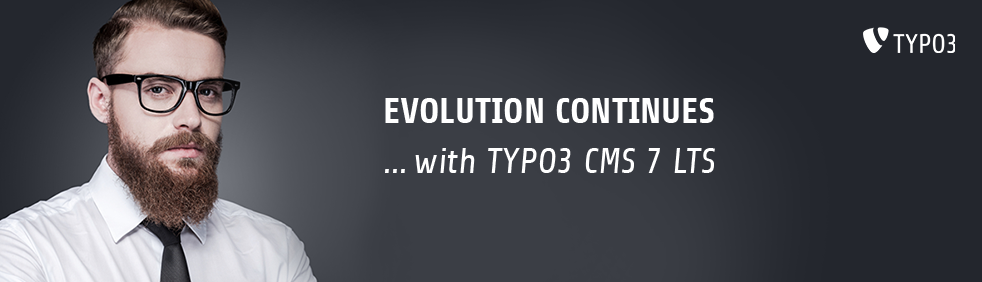
\includegraphics[width=0.95\linewidth]{Introduction/typo3cms76-banner.png}
	\end{figure}

\end{frame}

% ------------------------------------------------------------------------------
% LTXE-SLIDE-START
% LTXE-SLIDE-UID:		47227649-cbb8db0b-a70034c1-3dc92bc6
% LTXE-SLIDE-ORIGIN:	737c8e9b-4ae60e26-6975ea72-21146dd0 English
% LTXE-SLIDE-ORIGIN:	07f94e22-95cf3db6-373b81e0-4b00bb57 German
% LTXE-SLIDE-TITLE:		System Requirements
% ------------------------------------------------------------------------------
\begin{frame}[fragile]
	\frametitle{Introduction}
	\framesubtitle{System Requirements}

	\begin{itemize}
		\item PHP*:\tabto{2.2cm}v5.5.0 - v5.6.x
		\item MySQL:\tabto{2.2cm}v5.5.x - v5.6.x (no strict mode)
		\item Disk space:\tabto{2.2cm}min 200 MB
		\item PHP settings:

			\begin{itemize}
				\item memory\_limit >= 128M
				\item max\_execution\_time >= 240s
				\item compilation option \texttt{--disable-ipv6} must \underline{not} be used
			\end{itemize}

		\item Backend requires IE >= 9 or any other modern browser

	\end{itemize}

	\vspace{1cm}

	*) Further details: \href{http://typo3.org/news/article/php-minimum-requirements-for-typo3-cms-7/}{PHP Minimum Requirements for TYPO3 CMS 7}

\end{frame}

% ------------------------------------------------------------------------------
% LTXE-SLIDE-START
% LTXE-SLIDE-UID:		7f96aaa8-87411a0e-3b2be2b7-b5ec7c3f
% LTXE-SLIDE-ORIGIN:	90d2d3d1-f9d57661-dd01143b-10630416 English
% LTXE-SLIDE-ORIGIN:	79b3ee12-a96f5128-178eb0a1-52534b81 German
% LTXE-SLIDE-TITLE:		Development And Release Timeline
% ------------------------------------------------------------------------------
\begin{frame}[fragile]
	\frametitle{Introduction}
	\framesubtitle{Development and Release Timeline}

	\begin{figure}
		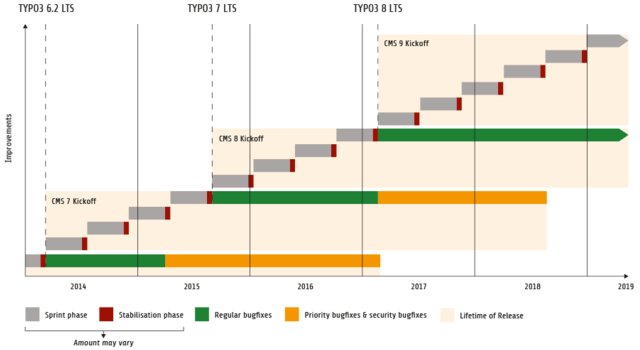
\includegraphics[width=0.90\linewidth]{Introduction/ReleaseAgenda.png}
	\end{figure}

\end{frame}

% ------------------------------------------------------------------------------
% LTXE-SLIDE-START
% LTXE-SLIDE-UID:		6564d2a4-7ce85907-c24dd475-90de5343
% LTXE-SLIDE-ORIGIN:	13e0fd6a-fa50d02d-c15c4af0-f3996926 English
% LTXE-SLIDE-ORIGIN:	89509115-eb2b6501-4bf03801-c53e7c0c German
% LTXE-SLIDE-TITLE:		TYPO3 CMS Roadmap
% ------------------------------------------------------------------------------
\begin{frame}[fragile]
	\frametitle{Introduction}
	\framesubtitle{TYPO3 CMS Roadmap}

	Release dates and their primary focus:

	\begin{itemize}
		\item v7.0 \tabto{1.1cm}02/Dez/2014\tabto{3.4cm}Backend Overhaul Vol 1
		\item v7.1 \tabto{1.1cm}24/Feb/2015\tabto{3.4cm}Core Cleanup \& Streamlining
		\item v7.2 \tabto{1.1cm}28/Apr/2015\tabto{3.4cm}Frontend
		\item v7.3 \tabto{1.1cm}16/Jun/2015\tabto{3.4cm}Package Ecosystem, Composer
		\item v7.4 \tabto{1.1cm}04/Aug/2015\tabto{3.4cm}Backend Overhaul Vol 2
		\item v7.5 \tabto{1.1cm}29/Sep/2015\tabto{3.4cm}Finalization

		\item
			\begingroup
				\color{typo3orange}
					v7 LTS \tabto{1.1cm}10/Nov/2015\tabto{3.4cm}\textbf{TYPO3 CMS 7 LTS} (Long Term Support)
			\endgroup

	\end{itemize}

	\smaller
		\url{https://typo3.org/typo3-cms/roadmap/}\newline
		\url{http://typo3.org/news/article/embrace-and-innovate-typo3-cms-7/}
	\normalsize

\end{frame}

% ------------------------------------------------------------------------------
% LTXE-SLIDE-START
% LTXE-SLIDE-UID:		9c8bd243-bc8474c1-d761afc2-f2817cba
% LTXE-SLIDE-ORIGIN:	06c6100a-69216610-618bde63-bbdc4eef English
% LTXE-SLIDE-ORIGIN:	8ac7908b-f1a64895-d12d437b-9309b07b German
% LTXE-SLIDE-TITLE:		Installation
% ------------------------------------------------------------------------------
\begin{frame}[fragile]
	\frametitle{Introduction}
	\framesubtitle{Installation}

	\begin{itemize}
		\item Official installation procedure under Linux/Mac OS X\newline
			(DocumentRoot for example \texttt{/var/www/site/htdocs}):
		\begin{lstlisting}
			$ cd /var/www/site
			$ wget --content-disposition get.typo3.org/7.6
			$ tar xzf typo3_src-7.6.0.tar.gz
			$ cd htdocs
			$ ln -s ../typo3_src-7.6.0 typo3_src
			$ ln -s typo3_src/index.php
			$ ln -s typo3_src/typo3
			$ touch FIRST_INSTALL
		\end{lstlisting}

		\item Symbolic links under Microsoft Windows:

			\begin{itemize}
				\item Use \texttt{junction} under Windows XP/2000
				\item Use \texttt{mklink} under Windows Vista and Windows 7
			\end{itemize}

	\end{itemize}
\end{frame}

% ------------------------------------------------------------------------------
% LTXE-SLIDE-START
% LTXE-SLIDE-UID:		443dd4b6-c034513c-560f2833-77317627
% LTXE-SLIDE-ORIGIN:	e4b09ddf-4c0ea575-9e0900ad-b878899c English
% LTXE-SLIDE-ORIGIN:	d146f854-4fcfed01-7de68fce-c2599f7f German
% LTXE-SLIDE-TITLE:		Upgrade to TYPO3 CMS 7
% ------------------------------------------------------------------------------
\begin{frame}[fragile]
	\frametitle{Introduction}
	\framesubtitle{Upgrade to TYPO3 CMS 7.x}

	\begin{itemize}
		\item Upgrades only possible from TYPO3 CMS 6.2 LTS
		\item TYPO3 CMS < 6.2 should be updated to TYPO3 CMS 6.2 LTS first
	\end{itemize}

	\begin{itemize}

		\item Upgrade instructions:\newline
			\smaller\url{http://wiki.typo3.org/Upgrade#Upgrading_to_7.6}\normalsize
		\item Official TYPO3 guide "TYPO3 Installation and Upgrading":
			\smaller\url{http://docs.typo3.org/typo3cms/InstallationGuide}\normalsize
		\item General approach:
			\begin{itemize}
				\item Check minimum system requirements \small(PHP, MySQL, etc.)
				\item Review \textbf{deprecation\_*.log} in old TYPO3 instance
				\item Update all extensions to the latest version
				\item Deploy new sources and run Install Tool -> Upgrade Wizard
				\item Review startup module for backend users (optionally)
			\end{itemize}
	\end{itemize}

\end{frame}

% ------------------------------------------------------------------------------
